\newpage
\subsection{QuizziPedia::Front-End::Controllers}


\begin{figure}
	\centering
	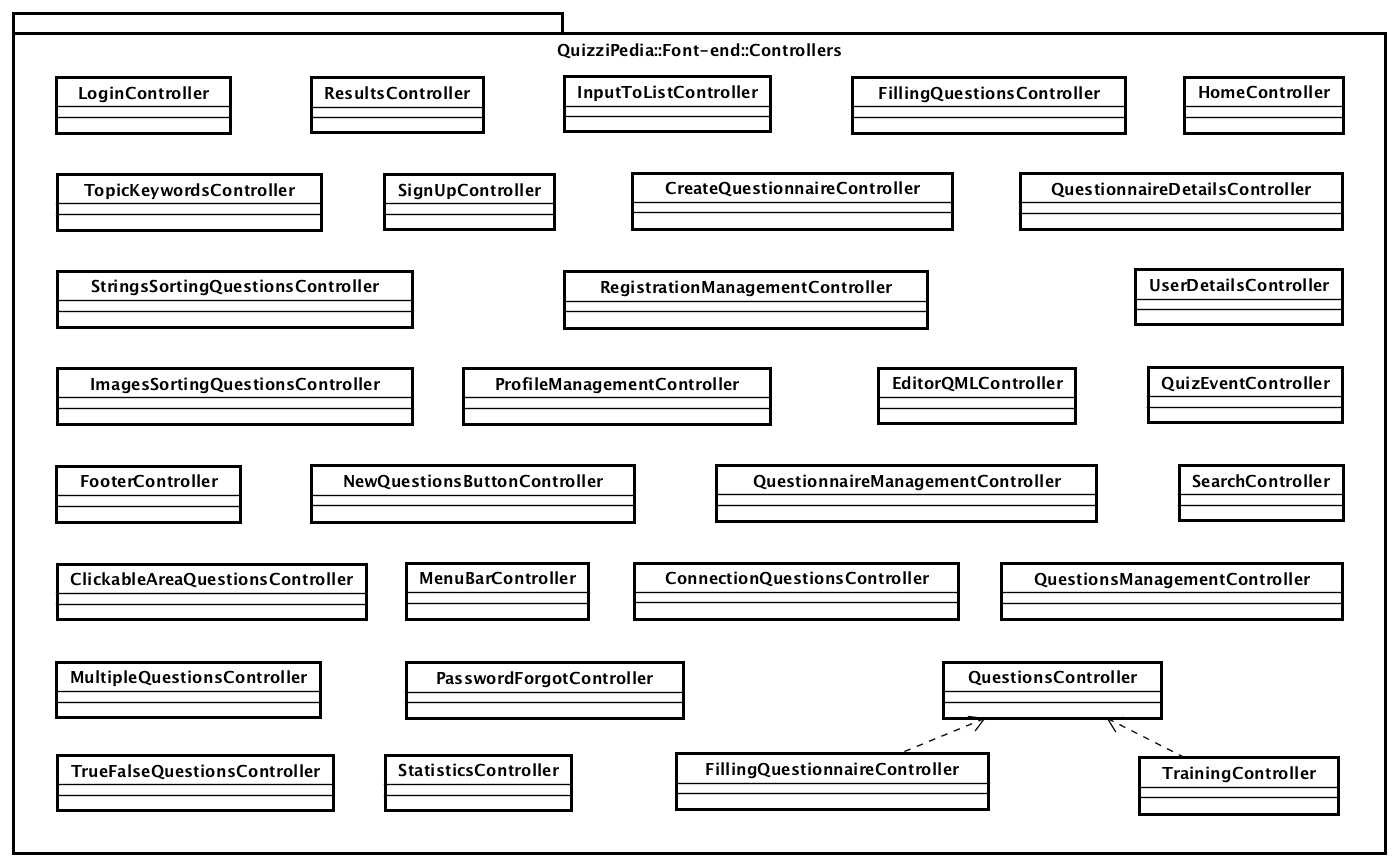
\includegraphics[scale=0.45]{UML/Package/QuizziPedia_Front-End_Controllers.png}
	\caption{QuizziPedia::Front-End::Controllers::SignUpController}
\end{figure}

\subsubsection{Informazioni generali}
\begin{itemize}
	\item \textbf{Descrizione}: package che contiene i controller individuati per la parte front-end dell'applicazione;
	\item \textbf{Padre:} \texttt{Front-End};
	\item \textbf{Interazione con altri componenti:}
	\begin{itemize}
		\item \texttt{Models} - package che contiene le classi model individuate;
		\item \texttt{Services} - package che contiene le classi services individuate.
	\end{itemize} 
\end{itemize}
\subsubsection{Classi}

\paragraph{QuizziPedia::Front-End::Controllers::LoginController}
\begin{figure}
	\centering
	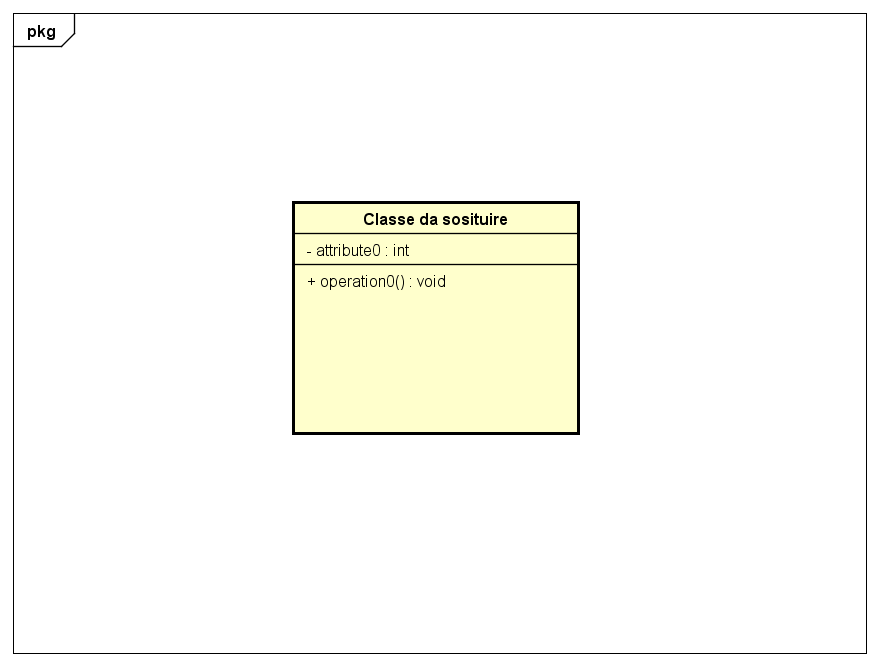
\includegraphics[scale=0.45]{UML/Classi/Front-End/Temporanea.png}
	\caption{QuizziPedia::Front-End::Controllers::LoginController}
\end{figure}
\begin{itemize}
	\item \textbf{Descrizione}: questa classe permette di gestire l'autenticazione dell'utente al sistema; 
	\item \textbf{Utilizzo}: fornisce le funzionalità di autenticazione al sistema, compresa la gestione di situazioni di errore autenticazione;
	\item \textbf{Relazione con altre classi:}
	\begin{itemize}
		\item \textit{IN} \texttt{LoginView}:  
		\item \textit{OUT} \texttt{LangService}:
		\item \textit{OUT} \texttt{AuthService}:
		\item \textit{OUT} \texttt{ErrorController}: 

	\end{itemize}
	\item \textbf{Attributi:}
	\begin{itemize}
		\item 
	\end{itemize}
	\item \textbf{Metodi:}
	\begin{itemize}
		\item 
	\end{itemize}
\end{itemize}

\paragraph{QuizziPedia::Front-End::Controllers::SignUpController}
\begin{figure}
	\centering
	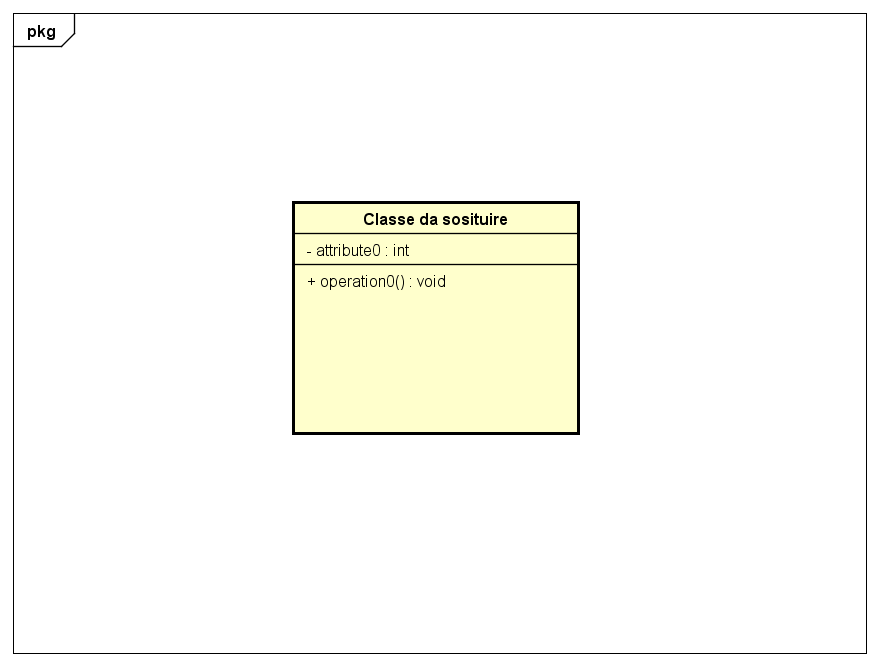
\includegraphics[scale=0.45]{UML/Classi/Front-End/Temporanea.png}
	\caption{QuizziPedia::Front-End::Controllers::SignUpController}
\end{figure}
\begin{itemize}
	\item \textbf{Descrizione}: questa classe permette di gestire la registrazione di un utente al sistema;
	\item \textbf{Utilizzo}: fornisce le funzionalità di registrazione di un utente al sistema;
	\item \textbf{Relazione con altre classi:}
	\begin{itemize}
		\item \textit{IN} \texttt{SignUpView}:
		\item \textit{OUT} \texttt{AuthService}: 
		\item \textit{OUT} \texttt{LangService}: 
		\item \textit{OUT} \texttt{ErrorController}:  
	\end{itemize}
	\item \textbf{Attributi:}
	\begin{itemize}
		\item 
	\end{itemize}
	\item \textbf{Metodi:}
	\begin{itemize}
		\item 
	\end{itemize}
\end{itemize}

\paragraph{QuizziPedia::Front-End::Controllers::HomeController}
\begin{figure}
	\centering
	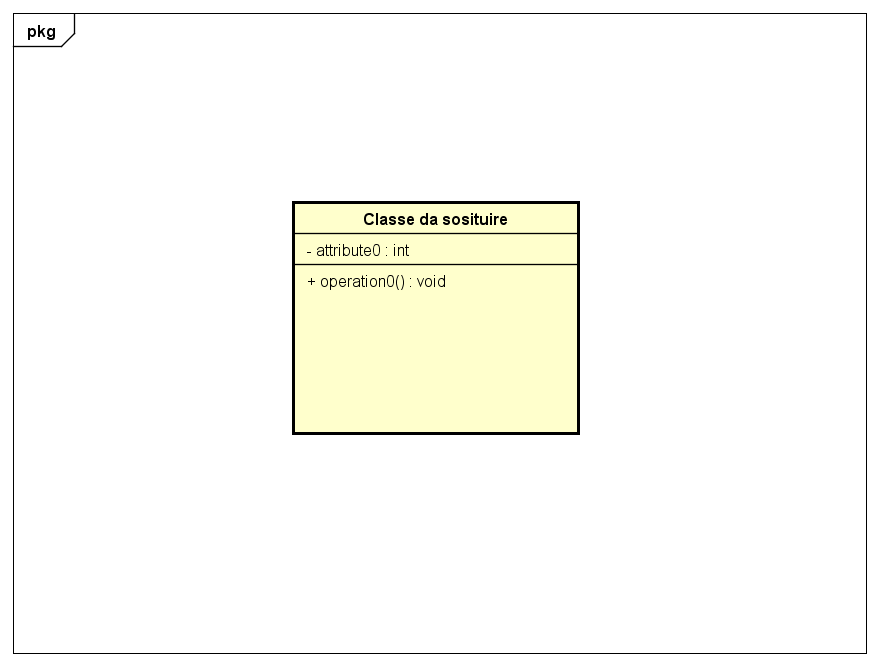
\includegraphics[scale=0.45]{UML/Classi/Front-End/Temporanea.png}
	\caption{QuizziPedia::Front-End::Controllers::HomeController}
\end{figure}
\begin{itemize}
	\item \textbf{Descrizione}: questa classe permette di gestire la home page;
	\item \textbf{Utilizzo}: fornisce tutte le informazioni da mostrare nella homepage;
	\item \textbf{Relazione con altre classi:}
	\begin{itemize}
		\item \textit{IN} \texttt{HomeView}: 
		\item \textit{OUT} \texttt{LangService}: 
	\end{itemize}
	\item \textbf{Attributi:}
	\begin{itemize}
		\item 
	\end{itemize}
	\item \textbf{Metodi:}
	\begin{itemize}
		\item 
	\end{itemize}
\end{itemize}

\paragraph{QuizziPedia::Front-End::Controllers::SearchController}
\begin{figure}
	\centering
	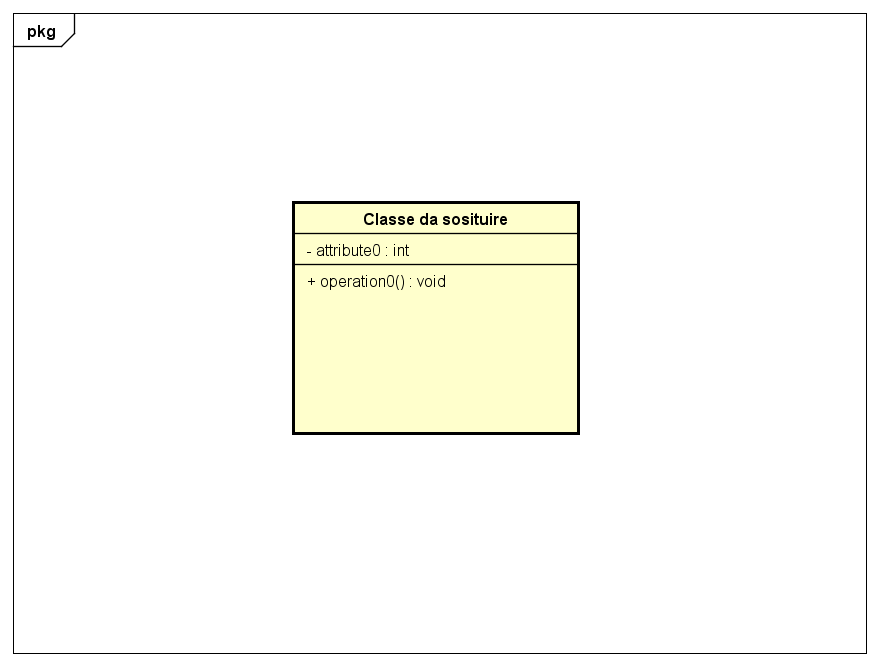
\includegraphics[scale=0.45]{UML/Classi/Front-End/Temporanea.png}
	\caption{QuizziPedia::Front-End::Controllers::SearchController}
\end{figure}
\begin{itemize}
	\item \textbf{Descrizione}: questa classe permette di gestire la ricerca di questionari e utenti all'interno dell'applicazione;
	\item \textbf{Utilizzo}: fornisce all'utente le funzionalità di ricerca per utenti e questionari;
	\item \textbf{Relazione con altre classi:}
	\begin{itemize}
		\item \textit{IN} \texttt{ErrorController}: 
		\item \textit{OUT} \texttt{UserDetailsService}: 
		\item \textit{OUT} \texttt{QuizService}: 
		\item \textit{OUT} \texttt{LangService}: 
	\end{itemize}
	\item \textbf{Attributi:}
	\begin{itemize}
		\item 
	\end{itemize}
	\item \textbf{Metodi:}
	\begin{itemize}
		\item 
	\end{itemize}
\end{itemize}

\paragraph{QuizziPedia::Front-End::Controllers::ProfileManagementController}
\begin{figure}
	\centering
	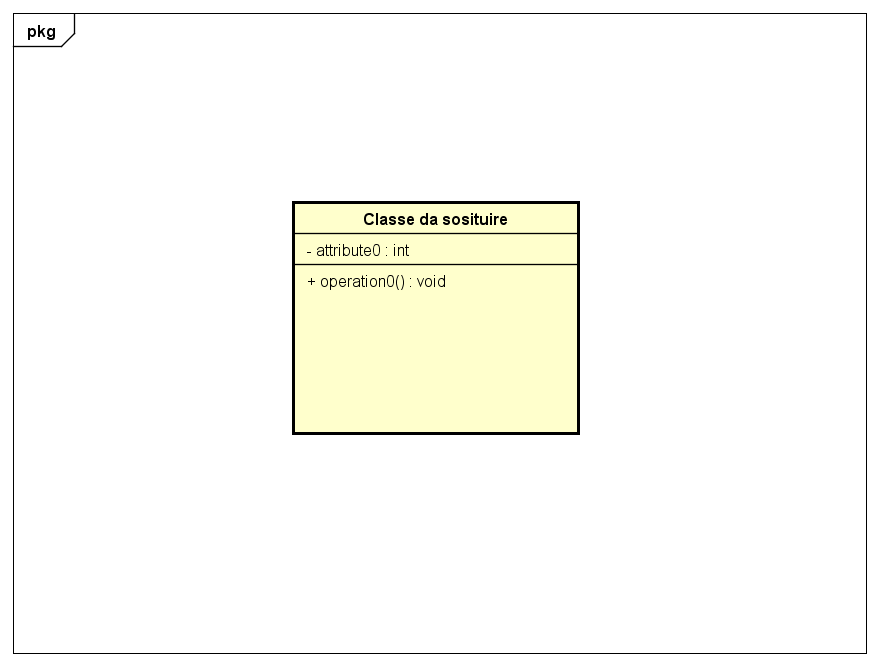
\includegraphics[scale=0.45]{UML/Classi/Front-End/Temporanea.png}
	\caption{QuizziPedia::Front-End::Controllers::ProfileManagementController}
\end{figure}
\begin{itemize}
	\item \textbf{Descrizione}: questa classe permette di gestire il profilo personale di un utente; 
	\item \textbf{Utilizzo}: fornisce le funzionalità all'utente per poter gestire i propri dati;
	\item \textbf{Relazione con altre classi:}
	\begin{itemize}
		\item \textit{IN} \texttt{ProfileManagementView}:  
		\item \textit{OUT} \texttt{UserDetailsService}: 
		\item \textit{OUT} \texttt{LangService}: 
	\end{itemize}
	\item \textbf{Attributi:}
	\begin{itemize}
		\item 
	\end{itemize}
	\item \textbf{Metodi:}
	\begin{itemize}
		\item 
	\end{itemize}
\end{itemize}

\paragraph{QuizziPedia::Front-End::Controllers::LogoutController}
\begin{figure}
	\centering
	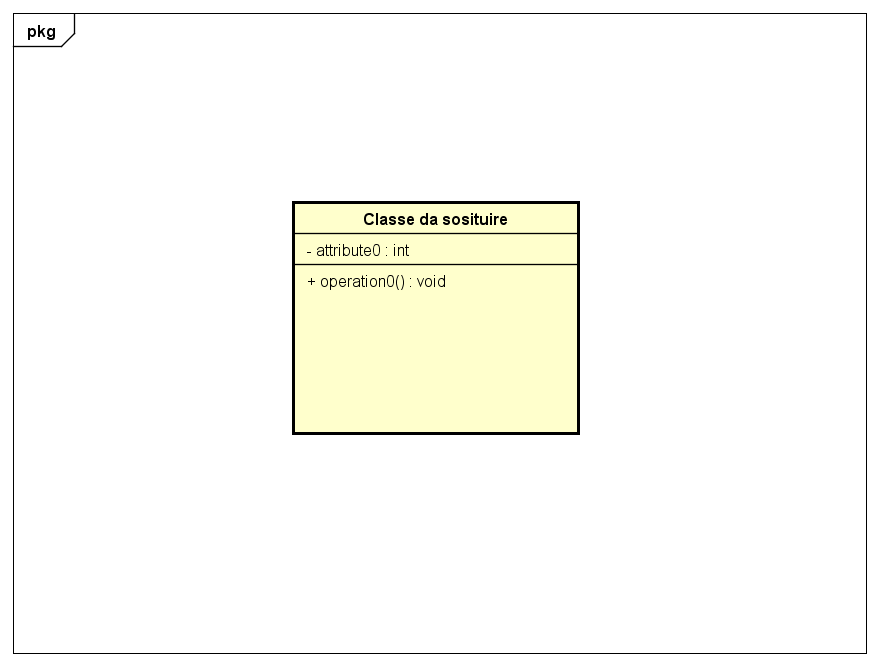
\includegraphics[scale=0.45]{UML/Classi/Front-End/Temporanea.png}
	\caption{QuizziPedia::Front-End::Controllers::LogoutController}
\end{figure}
\begin{itemize}
	\item \textbf{Descrizione}: questa classe permette di gestire la pagina di logout;
	\item \textbf{Utilizzo}: fornisce la funzionalità per effettuare il logout dall'applicazione;
	\item \textbf{Relazione con altre classi:}
	\begin{itemize}
		\item \textit{OUT} \texttt{MenuDirective}:
		\item \textit{OUT} \texttt{AuthService}: 
		\item \textit{OUT} \texttt{LangService}:
	\end{itemize}
	\item \textbf{Attributi:}
	\begin{itemize}
		\item 
	\end{itemize}
	\item \textbf{Metodi:}
	\begin{itemize}
		\item 
	\end{itemize}
\end{itemize}

\paragraph{QuizziPedia::Front-End::Controllers::PasswordForgotController}
\begin{figure}
	\centering
	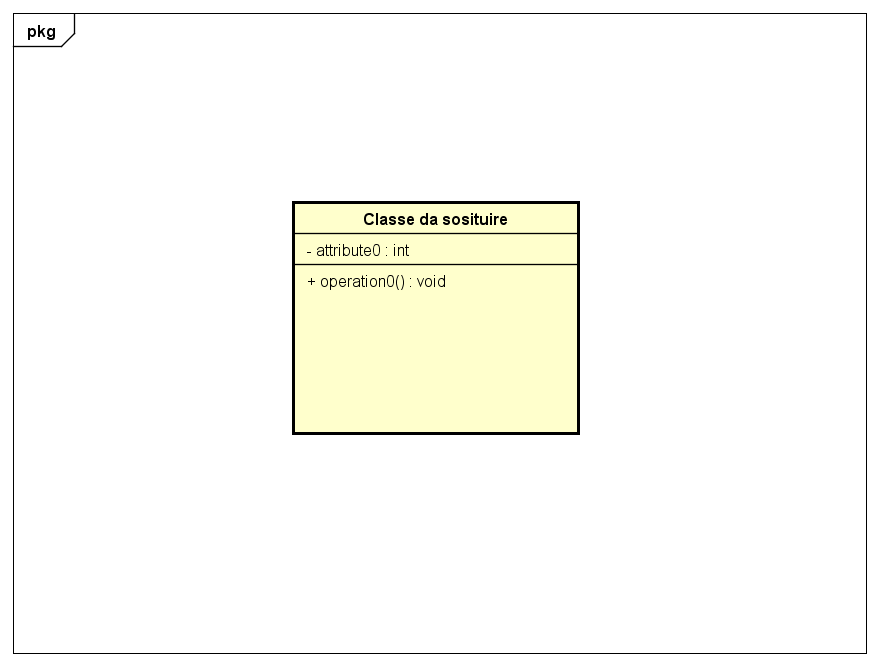
\includegraphics[scale=0.45]{UML/Classi/Front-End/Temporanea.png}
	\caption{QuizziPedia::Front-End::Controllers::PasswordForgotController}
\end{figure}
\begin{itemize}
	\item \textbf{Descrizione}: questa classe permette di gestire il ripristino della password dimenticata;
	\item \textbf{Utilizzo}: fornisce tutte le funzionalità per ripristinare la password dopo aver verificato l'identità dell'utente;
	\item \textbf{Relazione con altre classi:}
	\begin{itemize}
		\item \textit{IN} \texttt{PasswordForgotView}: 
		\item \textit{OUT} \texttt{AuthService}: 
		\item \textit{OUT} \texttt{LangService}: 
		\item \textit{OUT} \texttt{ErrorController}: 
	\end{itemize}
	\item \textbf{Attributi:}
	\begin{itemize}
		\item 
	\end{itemize}
	\item \textbf{Metodi:}
	\begin{itemize}
		\item 
	\end{itemize}
\end{itemize}

\paragraph{QuizziPedia::Front-End::Controllers::TrueFalseQuestionsController}
\begin{figure}
	\centering
	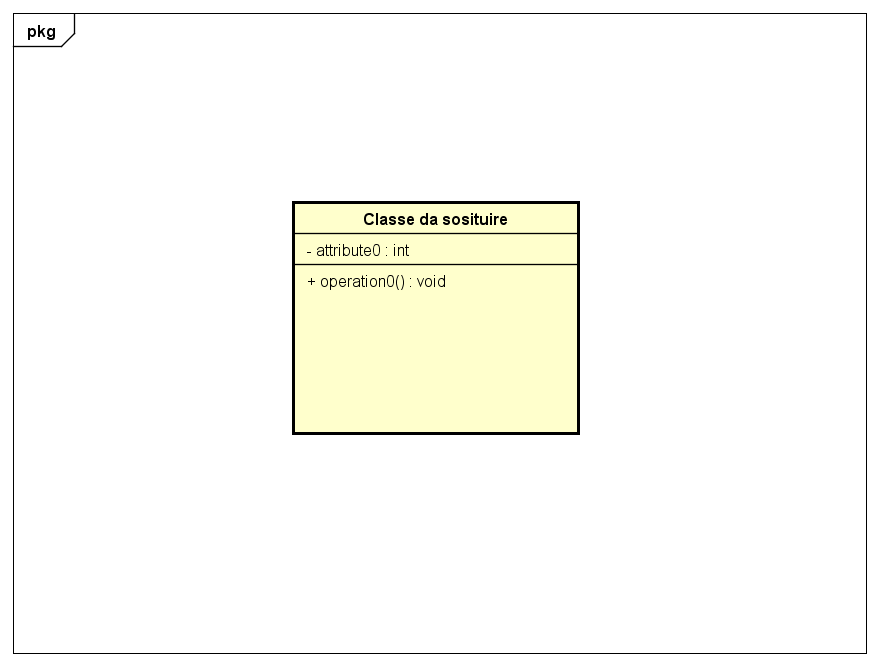
\includegraphics[scale=0.45]{UML/Classi/Front-End/Temporanea.png}
	\caption{QuizziPedia::Front-End::Controllers::TrueFalseQuestionsController}
\end{figure}
\begin{itemize}
	\item \textbf{Descrizione}: questa classe permette di gestire la creazione e la modifica di una domanda vero/falso;
	\item \textbf{Utilizzo}: fornisce le funzionalità per inserire una nuova domanda vero/falso nel database e per modificarne una esistente;
	\item \textbf{Relazione con altre classi:}
	\begin{itemize}
		\item \textit{IN} \texttt{TrueFalseQuestionsView}:  
		\item \textit{OUT} \texttt{LangService}: 
		\item \textit{OUT} \texttt{QuestionService}:
	\end{itemize}
	\item \textbf{Attributi:}
	\begin{itemize}
		\item 
	\end{itemize}
	\item \textbf{Metodi:}
	\begin{itemize}
		\item 
	\end{itemize}
\end{itemize}

\paragraph{QuizziPedia::Front-End::Controllers::MultiplyQuestionsController}
\begin{figure}
	\centering
	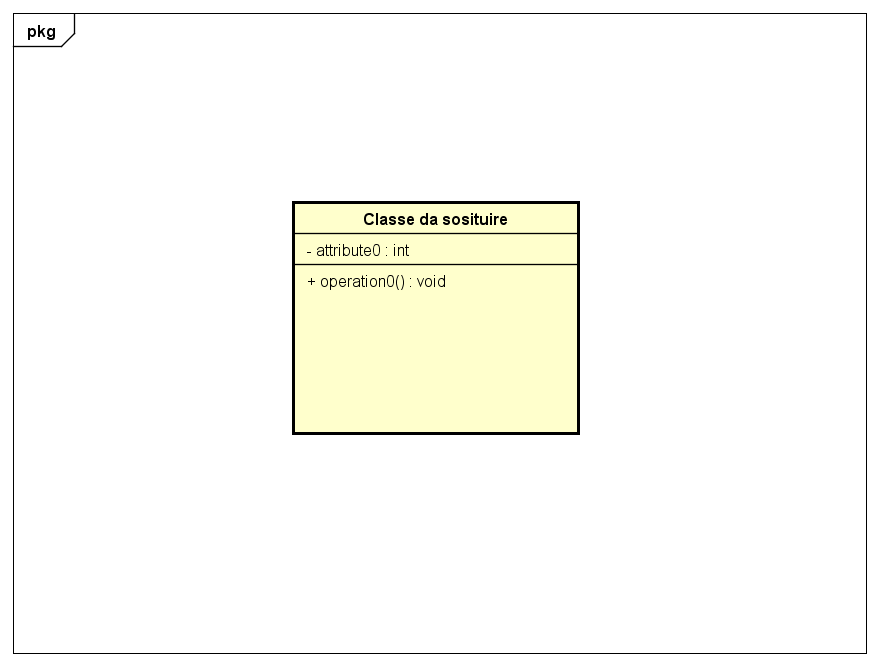
\includegraphics[scale=0.45]{UML/Classi/Front-End/Temporanea.png}
	\caption{QuizziPedia::Front-End::Controllers::MultiplyChoiceQuestion}
\end{figure}
\begin{itemize}
	\item \textbf{Descrizione}: questa classe permette di gestire la creazione e la modifica di una domanda a risposta multipla;
	\item \textbf{Utilizzo}: fornisce le funzionalità per inserire una nuova domanda a risposta multipla nel database e per modificarne una esistente;
	\item \textbf{Relazione con altre classi:}
	\begin{itemize}
		\item \textit{IN} \texttt{MultiplyQuestionsView}:  
		\item \textit{OUT} \texttt{LangService}: 
		\item \textit{OUT} \texttt{QuestionService}:
	\end{itemize}
	\item \textbf{Attributi:}
	\begin{itemize}
		\item 
	\end{itemize}
	\item \textbf{Metodi:}
	\begin{itemize}
		\item 
	\end{itemize}
\end{itemize}

\paragraph{QuizziPedia::Front-End::Controllers::ConnectionQuestionsController}
\begin{figure}
	\centering
	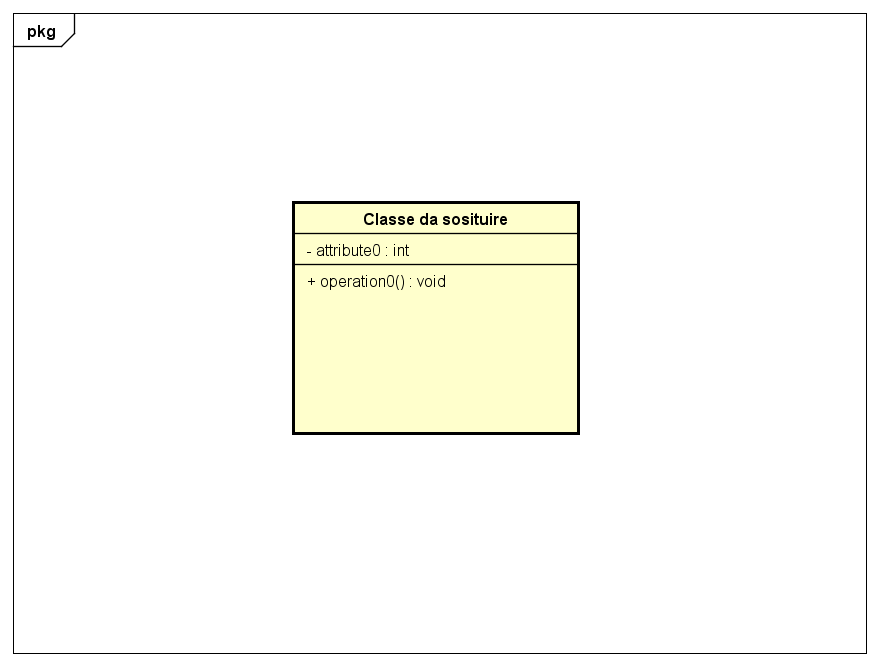
\includegraphics[scale=0.45]{UML/Classi/Front-End/Temporanea.png}
	\caption{QuizziPedia::Front-End::Controllers::ConnectionQuestionsController}
\end{figure}
\begin{itemize}
	\item \textbf{Descrizione}: questa classe permette di gestire la creazione e la modifica di una domanda a collegamento;
	\item \textbf{Utilizzo}: fornisce le funzionalità per inserire una nuova domanda a collegamento nel database e per modificarne una esistente;
	\item \textbf{Relazione con altre classi:}
	\begin{itemize}
		\item \textit{IN} \texttt{ConnectionQuestionsView}:  
		\item \textit{OUT} \texttt{LangService}: 
		\item \textit{OUT} \texttt{QuestionService}:
	\end{itemize}
	\item \textbf{Attributi:}
	\begin{itemize}
		\item 
	\end{itemize}
	\item \textbf{Metodi:}
	\begin{itemize}
		\item 
	\end{itemize}
\end{itemize}

\paragraph{QuizziPedia::Front-End::Controllers::ImagesSortingQuestionsController}
\begin{figure}
	\centering
	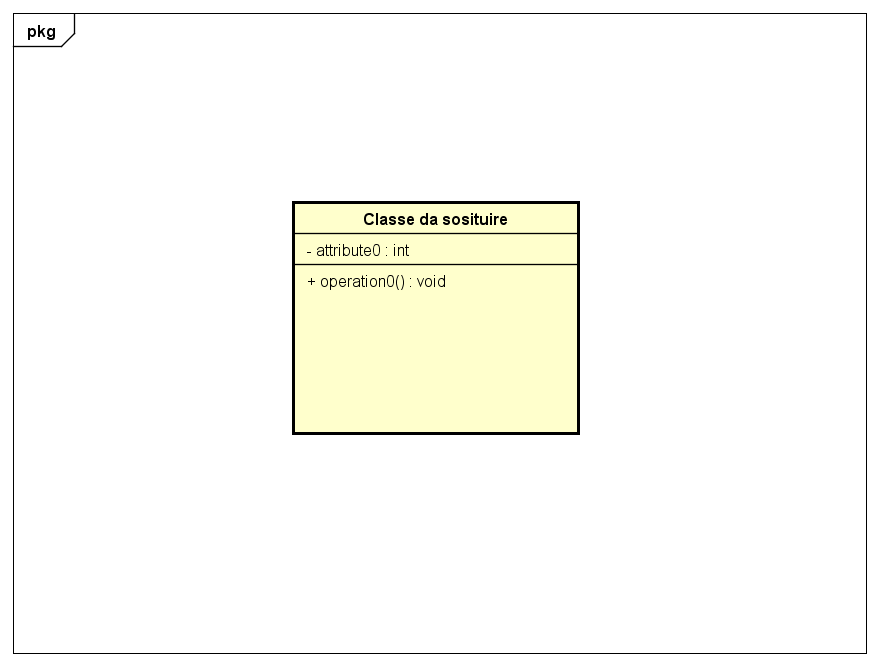
\includegraphics[scale=0.45]{UML/Classi/Front-End/Temporanea.png}
	\caption{QuizziPedia::Front-End::Controllers::ImagesSortingQuestionsController}
\end{figure}
\begin{itemize}
	\item \textbf{Descrizione}: questa classe permette di gestire la creazione e la modifica di una domanda a ordinamento immagini;
	\item \textbf{Utilizzo}: fornisce le funzionalità per inserire una nuova domanda a ordinamento immagini nel database e per modificarne una esistente;
	\item \textbf{Relazione con altre classi:}
	\begin{itemize}
		\item \textit{IN} \texttt{ImagesSortingQuestionsView}:  
		\item \textit{OUT} \texttt{LangService}: 
		\item \textit{OUT} \texttt{QuestionService}:
	\end{itemize}
	\item \textbf{Attributi:}
	\begin{itemize}
		\item 
	\end{itemize}
	\item \textbf{Metodi:}
	\begin{itemize}
		\item 
	\end{itemize}
\end{itemize}

\paragraph{QuizziPedia::Front-End::Controllers::StringsSortingQuestionsController}
\begin{figure}
	\centering
	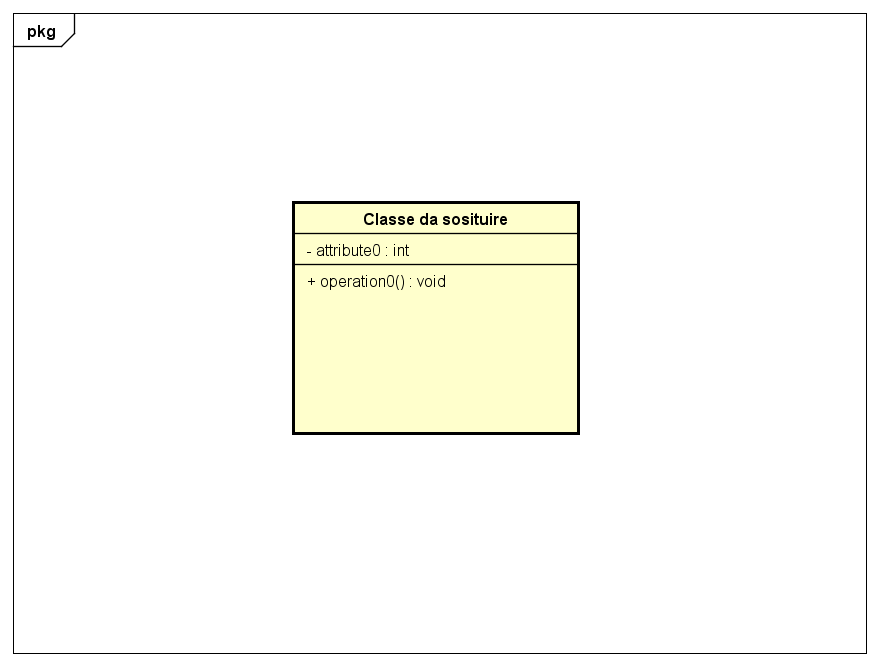
\includegraphics[scale=0.45]{UML/Classi/Front-End/Temporanea.png}
	\caption{QuizziPedia::Front-End::Controllers::StringsSortingQuestionsController}
\end{figure}
\begin{itemize}
	\item \textbf{Descrizione}: questa classe permette di gestire la creazione e la modifica di una domanda a ordinamento di stringhe;
	\item \textbf{Utilizzo}: fornisce le funzionalità per inserire una nuova domanda a ordinamento di stringhe nel database e per modificarne una esistente;
	\item \textbf{Relazione con altre classi:}
	\begin{itemize}
		\item \textit{IN} \texttt{StringsSortingQuestionsView}:  
		\item \textit{OUT} \texttt{LangService}: 
		\item \textit{OUT} \texttt{QuestionService}:
	\end{itemize}
	\item \textbf{Attributi:}
	\begin{itemize}
		\item 
	\end{itemize}
	\item \textbf{Metodi:}
	\begin{itemize}
		\item 
	\end{itemize}
\end{itemize}

\paragraph{QuizziPedia::Front-End::Controllers::FillingQuestionsController}
\begin{figure}
	\centering
	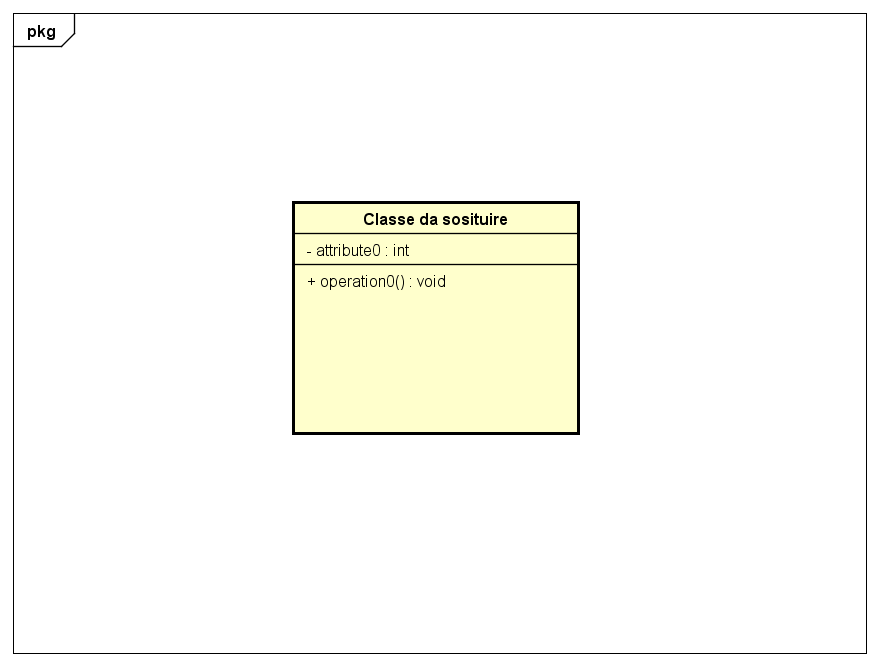
\includegraphics[scale=0.45]{UML/Classi/Front-End/Temporanea.png}
	\caption{QuizziPedia::Front-End::Controllers::FillingQuestionsController}
\end{figure}
\begin{itemize}
	\item \textbf{Descrizione}: questa classe permette di gestire la creazione e la modifica di una domanda a riempimento di spazi;
	\item \textbf{Utilizzo}: fornisce le funzionalità per inserire una nuova domanda ariempimento di spazi nel database e per modificarne una esistente;
	\item \textbf{Relazione con altre classi:}
	\begin{itemize}
		\item \textit{IN} \texttt{FillingQuestionsView}:  
		\item \textit{OUT} \texttt{LangService}: 
		\item \textit{OUT} \texttt{QuestionService}:
	\end{itemize}
	\item \textbf{Attributi:}
	\begin{itemize}
		\item 
	\end{itemize}
	\item \textbf{Metodi:}
	\begin{itemize}
		\item 
	\end{itemize}
\end{itemize}

\paragraph{QuizziPedia::Front-End::Controllers::ClickableAreaQuestionsController}
\begin{figure}
	\centering
	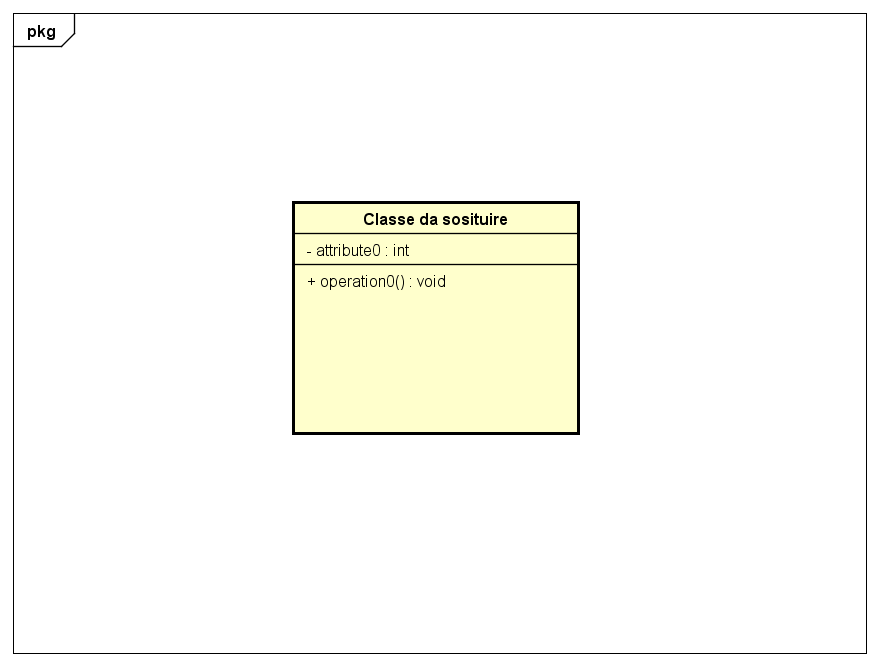
\includegraphics[scale=0.45]{UML/Classi/Front-End/Temporanea.png}
	\caption{QuizziPedia::Front-End::Controllers::ClickableAreaQuestionsController}
\end{figure}
\begin{itemize}
	\item \textbf{Descrizione}: questa classe permette di gestire la creazione e la modifica di una domanda ad area cliccabile;
	\item \textbf{Utilizzo}: fornisce le funzionalità per inserire una nuova domanda ad area cliccabile nel database e per modificarne una esistente;
	\item \textbf{Relazione con altre classi:}
	\begin{itemize}
		\item \textit{IN} \texttt{ClickableAreaQuestionsView}:  
		\item \textit{OUT} \texttt{LangService}: 
		\item \textit{OUT} \texttt{QuestionService}:
	\end{itemize}
	\item \textbf{Attributi:}
	\begin{itemize}
		\item 
	\end{itemize}
	\item \textbf{Metodi:}
	\begin{itemize}
		\item 
	\end{itemize}
\end{itemize}

\paragraph{QuizziPedia::Front-End::Controllers::EditorQMLController}
\begin{figure}
	\centering
	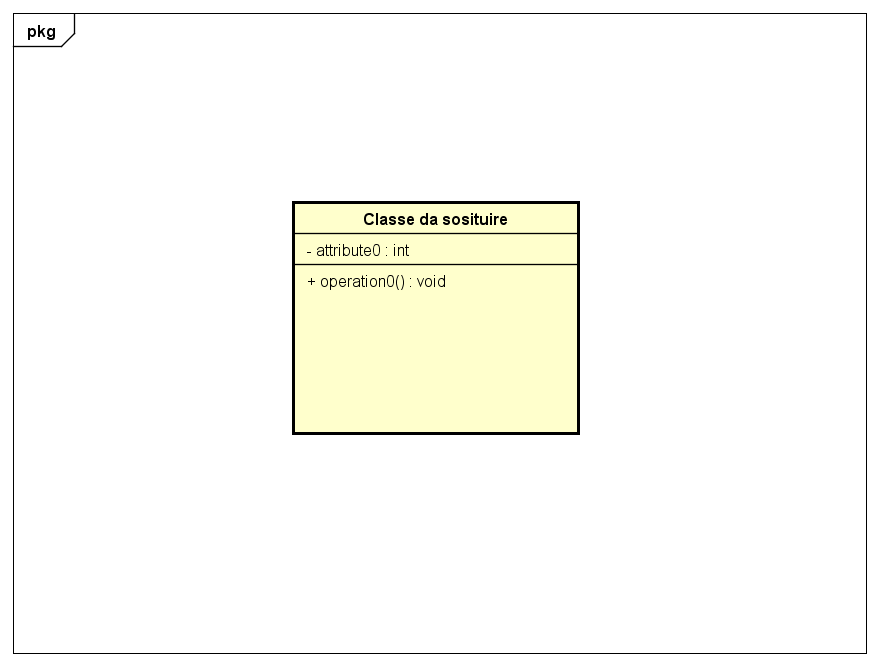
\includegraphics[scale=0.45]{UML/Classi/Front-End/Temporanea.png}
	\caption{QuizziPedia::Front-End::Controllers::EditorQMLController}
\end{figure}
\begin{itemize}
	\item \textbf{Descrizione}: questa classe permette di gestire la creazione e la modifica di domande create tramite editor QML;
	\item \textbf{Utilizzo}: fornisce le funzionalità per creare e modificare una domanda tramite editor QML;
	\item \textbf{Relazione con altre classi:}
	\begin{itemize}
		\item \textit{IN} \texttt{EditorQMLView}:  
		\item \textit{OUT} \texttt{LangService}: 
		\item \textit{OUT} \texttt{QuestionService}: 
	\end{itemize}
	\item \textbf{Attributi:}
	\begin{itemize}
		\item 
	\end{itemize}
	\item \textbf{Metodi:}
	\begin{itemize}
		\item 
	\end{itemize}
\end{itemize}

\paragraph{QuizziPedia::Front-End::Controllers::QuestionsManagementController}
\begin{figure}
	\centering
	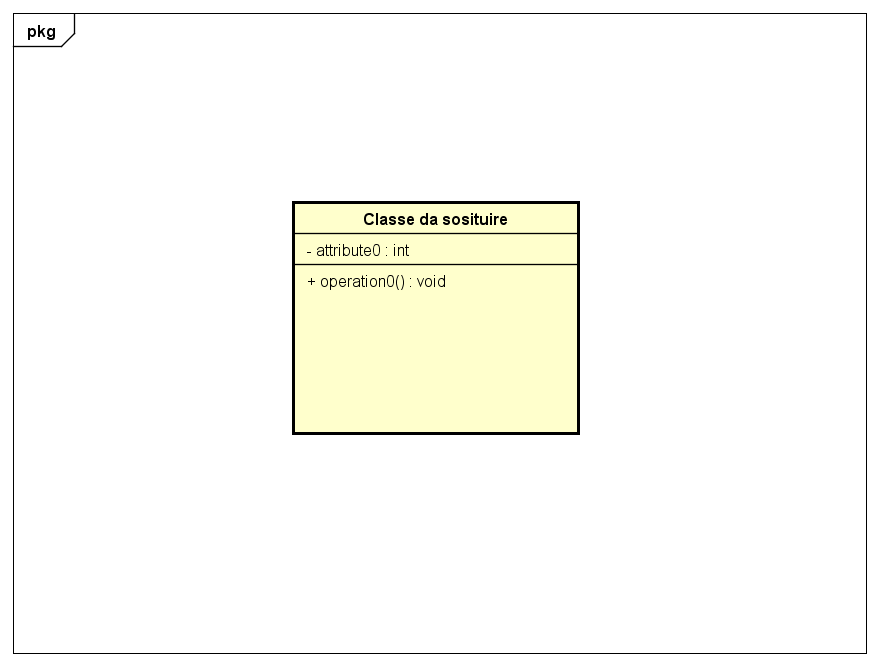
\includegraphics[scale=0.45]{UML/Classi/Front-End/Temporanea.png}
	\caption{QuizziPedia::Front-End::Controllers::QuestionsManagementController}
\end{figure}
\begin{itemize}
	\item \textbf{Descrizione}: questa classe permette di gestire di ottenere le domande create dall'utente;
	\item \textbf{Utilizzo}: fornisce le funzionalità per richiedere al back-end le domande create dall'utente e mostrarle nella sua pagina personale; 
	\item \textbf{Relazione con altre classi:}
	\begin{itemize}
		\item \textit{IN} \texttt{QuestionsManagementView}:  
		\item \textit{OUT} \texttt{LangService}:
		\item \textit{OUT} \texttt{QuestionService}: 
	\end{itemize}
	\item \textbf{Attributi:}
	\begin{itemize}
		\item 
	\end{itemize}
	\item \textbf{Metodi:}
	\begin{itemize}
		\item 
	\end{itemize}
\end{itemize}

\paragraph{QuizziPedia::Front-End::Controllers::TrainingController}
\begin{figure}
	\centering
	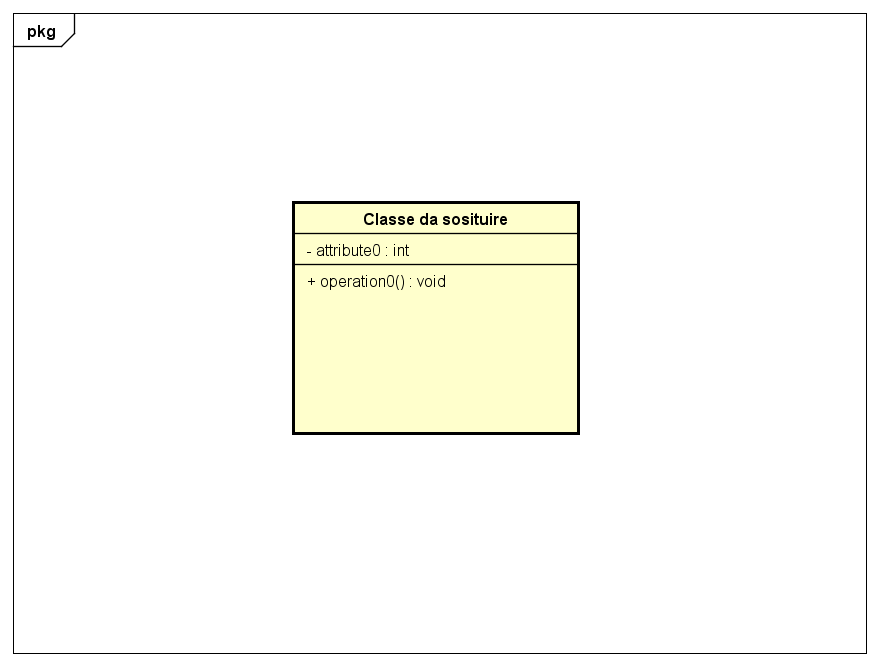
\includegraphics[scale=0.45]{UML/Classi/Front-End/Temporanea.png}
	\caption{QuizziPedia::Front-End::Controllers::TrainingController}
\end{figure}
\begin{itemize}
	\item \textbf{Descrizione}: questa classe permette di gestire la modalità allenamento sottoponendo all'utente le giuste domande adatte al suo livello;
	\item \textbf{Utilizzo}: fornisce le funzionalità per recuperare le domande che siano in accordo con il livello dell'utente;
	\item \textbf{Relazione con altre classi:}
	\begin{itemize}
		\item \textit{IN} \texttt{TrainingView}: 
		\item \textit{IN} \texttt{TrainingSetUpTemplate}:
		\item \textit{OUT} \texttt{LangService}:  
	\end{itemize}
	\item \textbf{Attributi:}
	\begin{itemize}
		\item 
	\end{itemize}
	\item \textbf{Metodi:}
	\begin{itemize}
		\item 
	\end{itemize}
\end{itemize}

\paragraph{QuizziPedia::Front-End::Controllers::FillingQuestionnaireController}
\begin{figure}
	\centering
	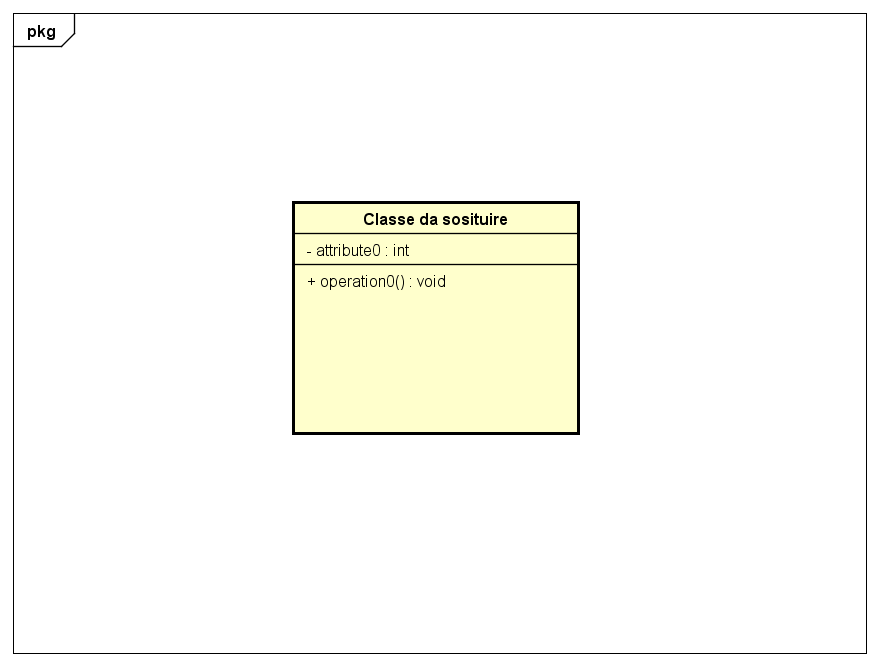
\includegraphics[scale=0.45]{UML/Classi/Front-End/Temporanea.png}
	\caption{QuizziPedia::Front-End::Controllers::FillingQuestionnaireController}
\end{figure}
\begin{itemize}
	\item \textbf{Descrizione}: questa classe permette di gestire la compilazione del questionario;
	\item \textbf{Utilizzo}: fornisce le funzionalità per compilare un questionario e per gestire il cambio di domanda;
	\item \textbf{Relazione con altre classi:}
	\begin{itemize}
		\item \textit{IN} \texttt{FillingQuestionnaireView}:  
		\item \textit{IN} \texttt{InfoQuestionnaireTemplate}: 
		\item \textit{OUT} \texttt{LangService}: 
		\item \textit{OUT} \texttt{QuizService}: 
	\end{itemize}
	\item \textbf{Attributi:}
	\begin{itemize}
		\item 
	\end{itemize}
	\item \textbf{Metodi:}
	\begin{itemize}
		\item 
	\end{itemize}
\end{itemize}

\paragraph{QuizziPedia::Front-End::Controllers::TemplateQuestionnaireController}
\begin{figure}
	\centering
	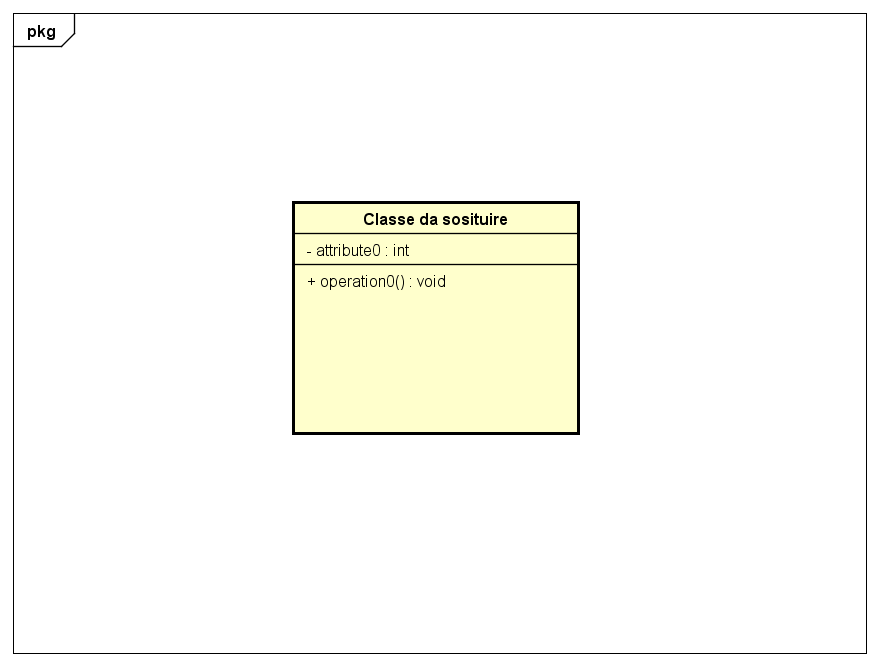
\includegraphics[scale=0.45]{UML/Classi/Front-End/Temporanea.png}
	\caption{QuizziPedia::Front-End::Controllers::TemplateQuestionnaireController}
\end{figure}
\begin{itemize}
	\item \textbf{Descrizione}: questa classe permette di gestire la creazione di un questionario;
	\item \textbf{Utilizzo}: fornisce tutte le funzionalità per la creazione di un nuovo questionario e per la modifica di uno esistente;
	\item \textbf{Relazione con altre classi:}
	\begin{itemize}
		\item \textit{IN} \texttt{TemplateQuestionnaireView}:  
		\item \textit{OUT} \texttt{QuizService}: 
		\item \textit{OUT} \texttt{LangService}: 
	\end{itemize}
	\item \textbf{Attributi:}
	\begin{itemize}
		\item 
	\end{itemize}
	\item \textbf{Metodi:}
	\begin{itemize}
		\item 
	\end{itemize}
\end{itemize}

\paragraph{QuizziPedia::Front-End::Controllers::RegistrationManagementController}
\begin{figure}
	\centering
	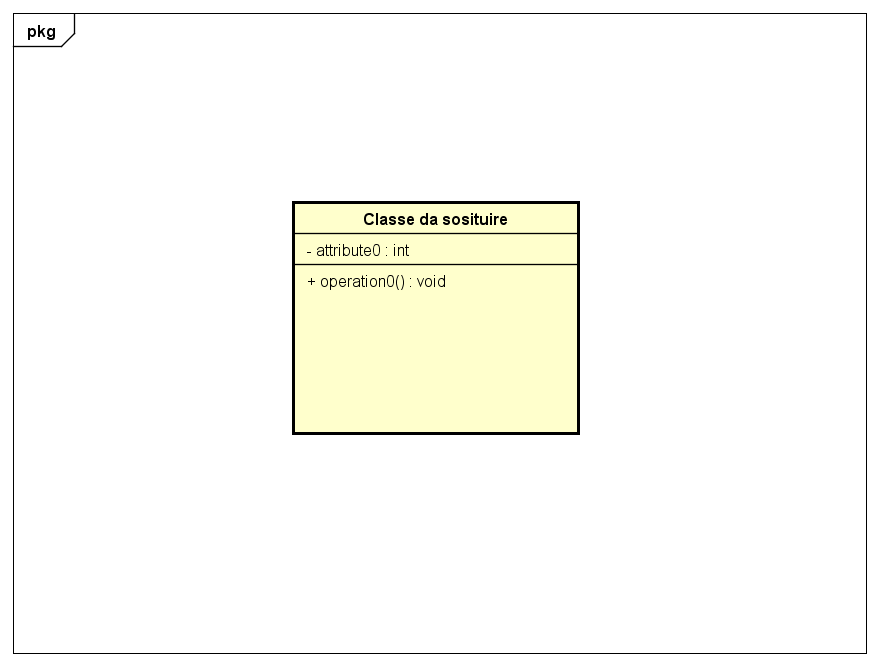
\includegraphics[scale=0.45]{UML/Classi/Front-End/Temporanea.png}
	\caption{QuizziPedia::Front-End::Controllers::RegistrationManagementController}
\end{figure}
\begin{itemize}
	\item \textbf{Descrizione}: questa classe permette di gestire le iscrizione degli utenti ai questionari;
	\item \textbf{Utilizzo}: fornisce le funzionalità di iscrizione ad un questionario;
	\item \textbf{Relazione con altre classi:}
	\begin{itemize}
		\item \textit{IN} \texttt{RegistratioManagementView}: 
		\item \textit{OUT} \texttt{QuizService}: 
		\item \textit{OUT} \texttt{LangService}: 
	\end{itemize}
	\item \textbf{Attributi:}
	\begin{itemize}
		\item 
	\end{itemize}
	\item \textbf{Metodi:}
	\begin{itemize}
		\item 
	\end{itemize}
\end{itemize}

\paragraph{QuizziPedia::Front-End::Controllers::ResultsController}
\begin{figure}
	\centering
	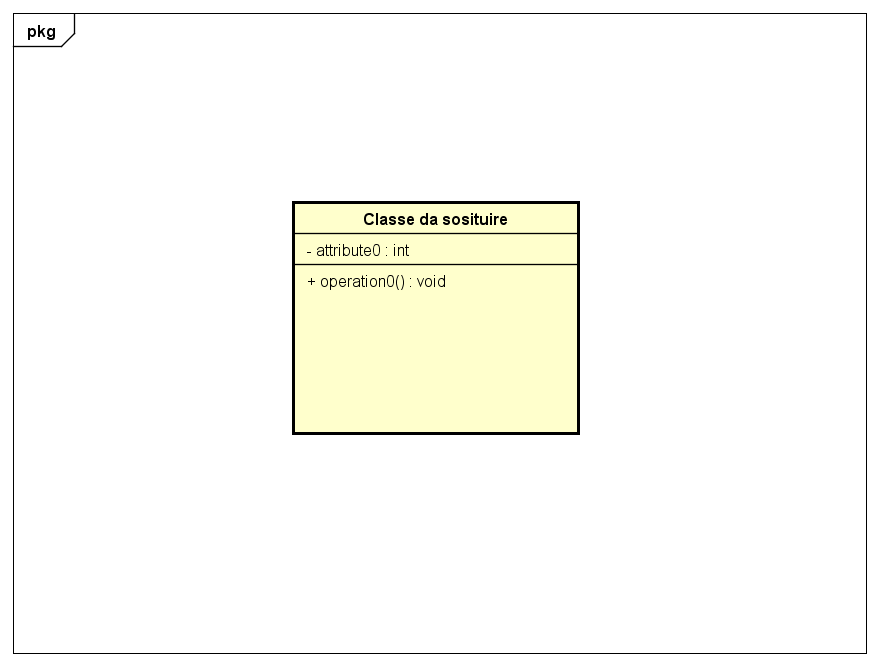
\includegraphics[scale=0.45]{UML/Classi/Front-End/Temporanea.png}
	\caption{QuizziPedia::Front-End::Controllers::ResultsController}
\end{figure}
\begin{itemize}
	\item \textbf{Descrizione}: questa classe permette di gestire i risultati della ricerca effettuata dall'utente;
	\item \textbf{Utilizzo}: fornisce le funzionalità per recuperare i dati dal back-end e mostrarli all'utente nella view;
	\item \textbf{Relazione con altre classi:}
	\begin{itemize}
		\item \textit{IN} \texttt{ResultsView}: 
		\item \textit{OUT} \texttt{QuizService}:
		\item \textit{OUT} \texttt{LangService}: 
	\end{itemize}
	\item \textbf{Attributi:}
	\begin{itemize}
		\item 
	\end{itemize}
	\item \textbf{Metodi:}
	\begin{itemize}
		\item 
	\end{itemize}
\end{itemize}

\paragraph{QuizziPedia::Front-End::Controllers::QuestionnaireManagementController}
\begin{figure}
	\centering
	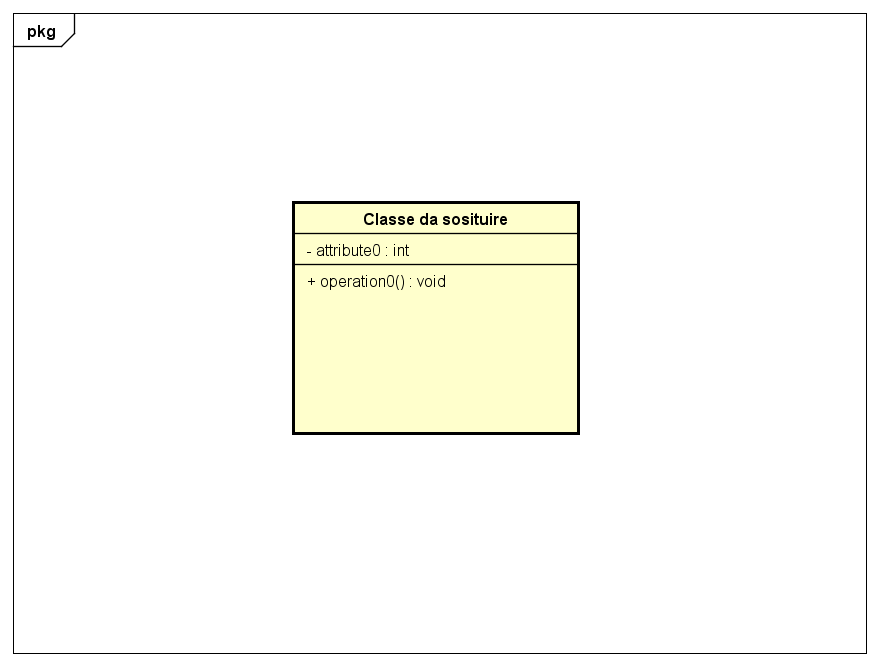
\includegraphics[scale=0.45]{UML/Classi/Front-End/Temporanea.png}
	\caption{QuizziPedia::Front-End::Controllers::QuestionnaireManagementController}
\end{figure}
\begin{itemize}
	\item \textbf{Descrizione}: questa classe permette di gestire tutti i questionari creati da un utente; 
	\item \textbf{Utilizzo}: fornisce le funzionalità per recuperare dal back-end tutti i questionari creati da un utente;
	\item \textbf{Relazione con altre classi:}
	\begin{itemize}
		\item \textit{IN} \texttt{QuestionnaireManagementeView}: 
		\item \textit{OUT} \texttt{QuizService}:
		\item \textit{OUT} \texttt{LangService}:
	\end{itemize}
	\item \textbf{Attributi:}
	\begin{itemize}
		\item 
	\end{itemize}
	\item \textbf{Metodi:}
	\begin{itemize}
		\item 
	\end{itemize}
\end{itemize}

\paragraph{QuizziPedia::Front-End::Controllers::MenuController}
\begin{figure}
	\centering
	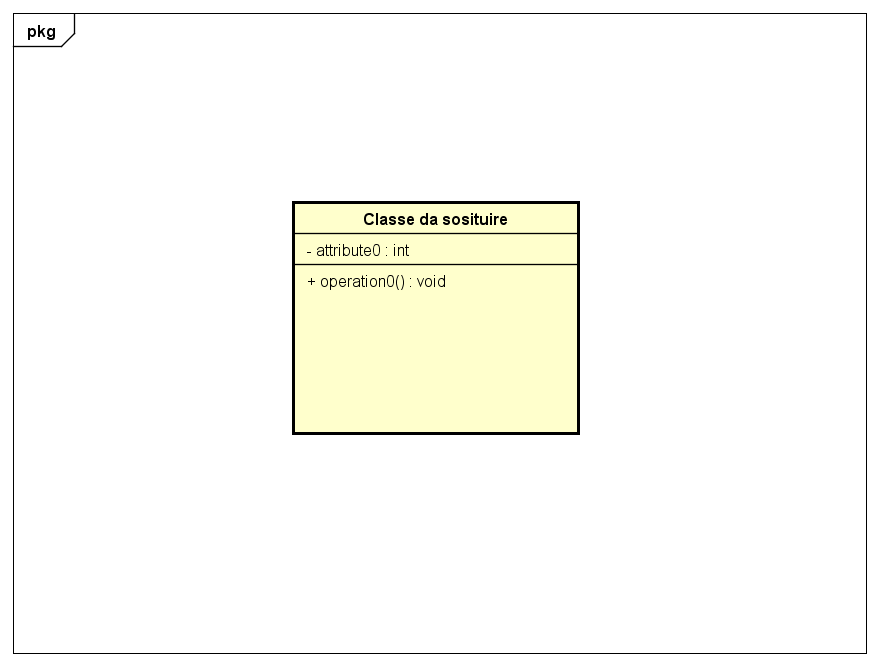
\includegraphics[scale=0.45]{UML/Classi/Front-End/Temporanea.png}
	\caption{QuizziPedia::Front-End::Controllers::MenuController}
\end{figure}
\begin{itemize}
	\item \textbf{Descrizione}: questa classe permette di gestire il menù fisso per ogni pagina;
	\item \textbf{Utilizzo}: fornisce le funzionalità per aggiornare, a seconda della pagina, il contenuto del menù;
	\item \textbf{Relazione con altre classi:}
	\begin{itemize}
		\item \textit{IN} \texttt{MenuDirective}:  
		\item \textit{OUT} \texttt{LangService}: 
	\end{itemize}
	\item \textbf{Attributi:}
	\begin{itemize}
		\item 
	\end{itemize}
	\item \textbf{Metodi:}
	\begin{itemize}
		\item 
	\end{itemize}
\end{itemize}

\paragraph{QuizziPedia::Front-End::Controllers::FooterController}
\begin{figure}
	\centering
	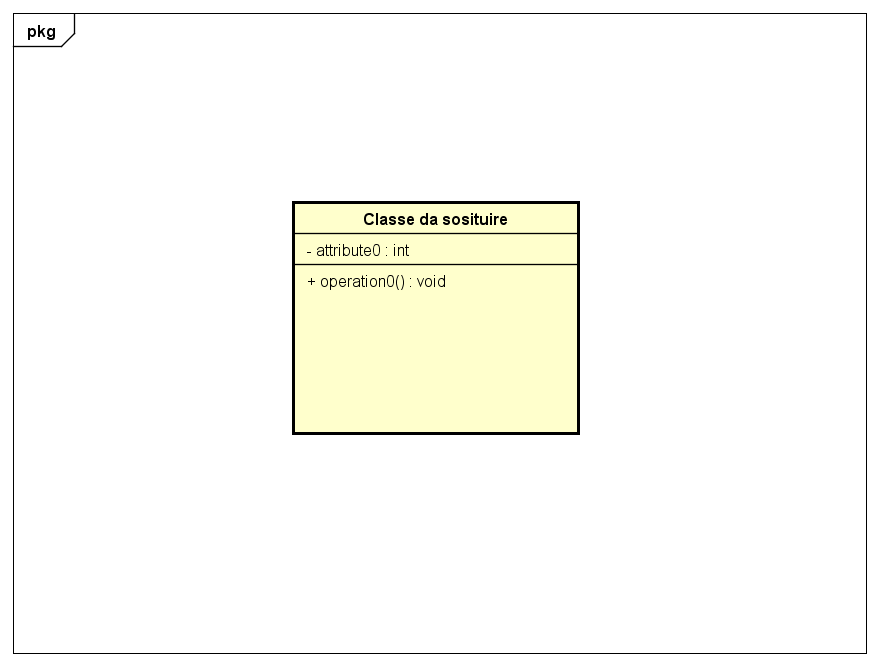
\includegraphics[scale=0.45]{UML/Classi/Front-End/Temporanea.png}
	\caption{QuizziPedia::Front-End::Controllers::FooterController}
\end{figure}
\begin{itemize}
	\item \textbf{Descrizione}: questa classe permette di gestire il footer dell'applicazione;
	\item \textbf{Utilizzo}: fornisce le funzionalità per recuperare le informazioni da mostrare nel footer;
	\item \textbf{Relazione con altre classi:}
	\begin{itemize}
		\item \textit{IN} \texttt{FooterDirective}:  
		\item \textit{OUT} \texttt{LangService}: 
	\end{itemize}
	\item \textbf{Attributi:}
	\begin{itemize}
		\item 
	\end{itemize}
	\item \textbf{Metodi:}
	\begin{itemize}
		\item 
	\end{itemize}
\end{itemize}

\paragraph{QuizziPedia::Front-End::Controllers::ErrorController}
\begin{figure}
	\centering
	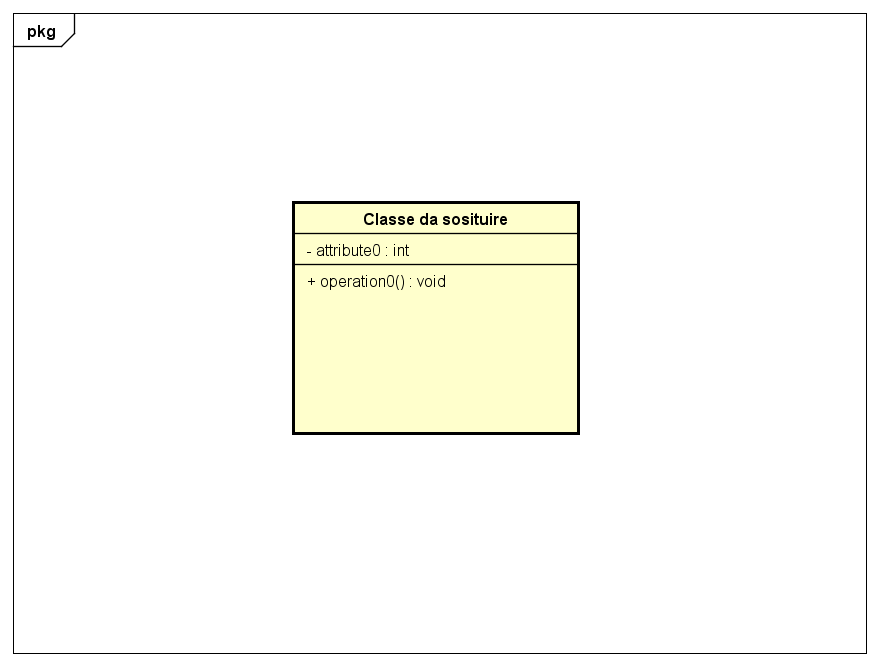
\includegraphics[scale=0.45]{UML/Classi/Front-End/Temporanea.png}
	\caption{QuizziPedia::Front-End::Controllers::ErrorController}
\end{figure}
\begin{itemize}
	\item \textbf{Descrizione}: questa classe permette di gestire tutti i messaggi di errore da mostrare all'utente;
	\item \textbf{Utilizzo}: fornisce le funzionalità che permettono di recuperare il giusto messaggio di errore ad ogni situazione anomala;
	\item \textbf{Relazione con altre classi:}
	\begin{itemize}
		\item \textit{IN} \texttt{ErrorDirective}: 
		\item \textit{IN} \texttt{LoginController}: 
		\item \textit{IN} \texttt{PasswordForgotController}: 
		\item \textit{IN} \texttt{SignUpController}: 
		\item \textit{IN} \texttt{SearchController}: 
		\item \textit{OUT} \texttt{LangService}: 
		\item \textit{OUT} \texttt{ErrorService}: 
	\end{itemize}
	\item \textbf{Attributi:}
	\begin{itemize}
		\item 
	\end{itemize}
	\item \textbf{Metodi:}
	\begin{itemize}
		\item 
	\end{itemize}
\end{itemize}

\paragraph{QuizziPedia::Front-End::Controllers::QuestionnaireDetailsController}
\begin{figure}
	\centering
	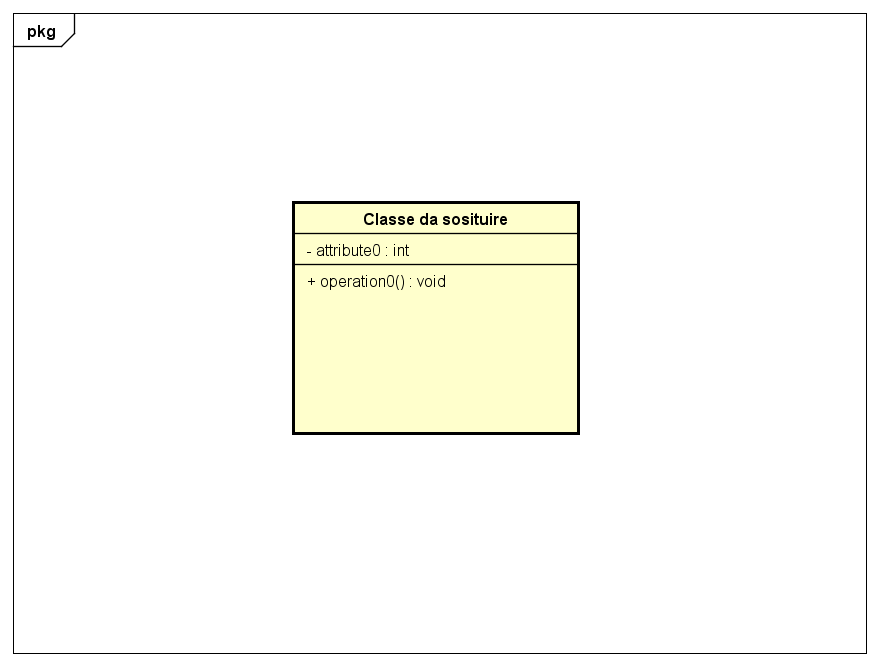
\includegraphics[scale=0.45]{UML/Classi/Front-End/Temporanea.png}
	\caption{QuizziPedia::Front-End::Controllers::QuestionnaireDetailsController}
\end{figure}
\begin{itemize}
	\item \textbf{Descrizione}: questa classe permette di gestire i dettagli di un questionario; 
	\item \textbf{Utilizzo}: fornisce le funzionalità per recuperare dal back-end i dettagli di un questionario creato da un utente al fine di poterli visualizzare nel suo profilo;
	\item \textbf{Relazione con altre classi:}
	\begin{itemize}
		\item \textit{IN} \texttt{QuestionnaireDetailsDirective}:
		\item \textit{OUT} \texttt{QuizService}: 
	\end{itemize}
	\item \textbf{Attributi:}
	\begin{itemize}
		\item 
	\end{itemize}
	\item \textbf{Metodi:}
	\begin{itemize}
		\item 
	\end{itemize}
\end{itemize}

\paragraph{QuizziPedia::Front-End::Controllers::UserDetailController}
\begin{figure}
	\centering
	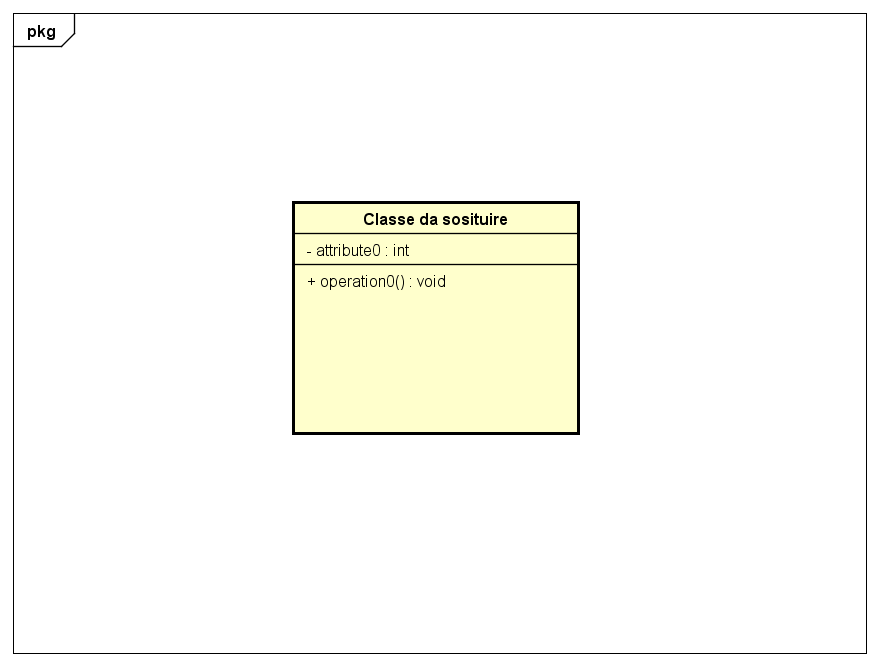
\includegraphics[scale=0.45]{UML/Classi/Front-End/Temporanea.png}
	\caption{QuizziPedia::Front-End::Controllers::UserDetailController}
\end{figure}
\begin{itemize}
	\item \textbf{Descrizione}: questa classe permette di gestire i dati di un utente;
	\item \textbf{Utilizzo}: fornisce le funzionalità per recuperare i dati di un utente, visualizzabili sia come dati personali dell'utente che ha effettuato l'accesso sia come risultato di una ricerca per utenti;
	\item \textbf{Relazione con altre classi:}
	\begin{itemize}
		\item \textit{IN} \texttt{UserDetailsDirective}: 
		\item \textit{OUT} \texttt{UserDetailsService}:

	\end{itemize}
	\item \textbf{Attributi:}
	\begin{itemize}
		\item 
	\end{itemize}
	\item \textbf{Metodi:}
	\begin{itemize}
		\item 
	\end{itemize}
\end{itemize}

\paragraph{QuizziPedia::Front-End::Controllers::QuestionsController}
\begin{figure}
	\centering
	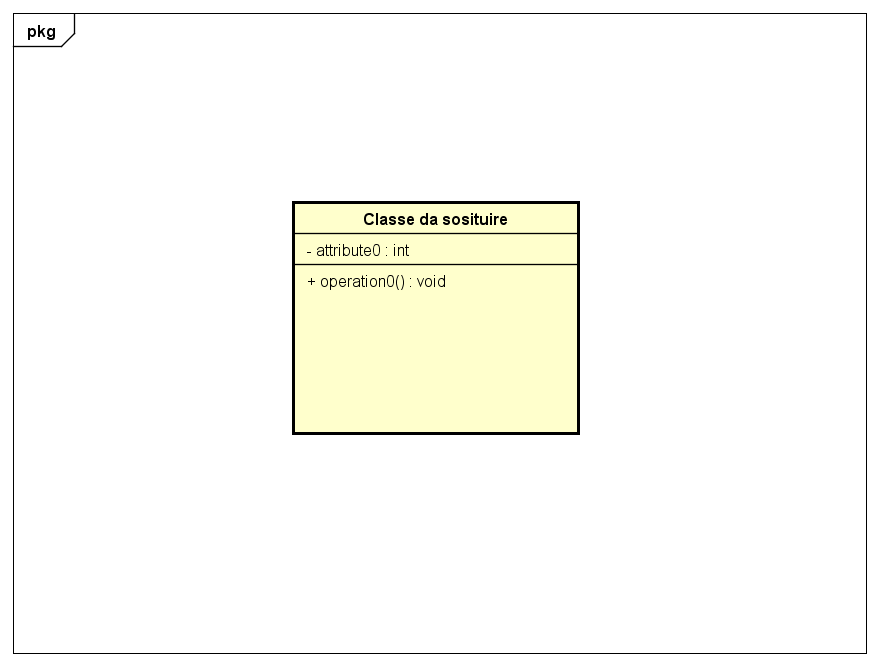
\includegraphics[scale=0.45]{UML/Classi/Front-End/Temporanea.png}
	\caption{QuizziPedia::Front-End::Controllers::QuestionsController}
\end{figure}
\begin{itemize}
	\item \textbf{Descrizione}: questa classe permette di gestire il recupero delle domande per poterle stampare nella modalità allenamento;
	\item \textbf{Utilizzo}: fornisce le funzionalità per il recupero delle domande esistenti nel database al fine di mostrarle durante la modalità allenamento nell'apposito template;
	\item \textbf{Relazione con altre classi:}
	\begin{itemize}
		\item \textit{IN} \texttt{HeaderTextQuestionTemplate}:  
		\item \textit{IN} \texttt{TrueFalseAnswerTemplate}:  
		\item \textit{IN} \texttt{MultipleChoiceAnswerTemplate}:  
		\item \textit{IN} \texttt{LinkingAnswerTemplate}:  
		\item \textit{IN} \texttt{SortImagesAnswerTemplate}:  
		\item \textit{IN} \texttt{SortTextAnswerTemplate}:  
		\item \textit{IN} \texttt{EmptyChoiceAnswerTemnplate}:  
		\item \textit{IN} \texttt{ClickableAnswerTemplate}:  
		\item \textit{OUT} \texttt{QuestionsServices}: 
	\end{itemize}
	\item \textbf{Attributi:}
	\begin{itemize}
		\item 
	\end{itemize}
	\item \textbf{Metodi:}
	\begin{itemize}
		\item 
	\end{itemize}
\end{itemize}

\paragraph{QuizziPedia::Front-End::Controllers::KeywordsController}
\begin{figure}
	\centering
	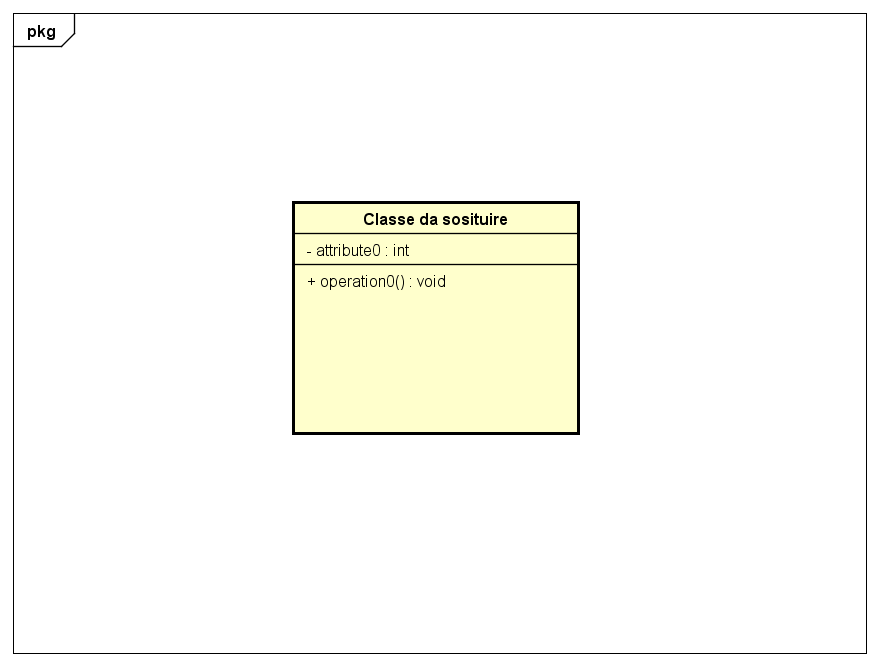
\includegraphics[scale=0.45]{UML/Classi/Front-End/Temporanea.png}
	\caption{QuizziPedia::Front-End::Controllers::KeywordsController}
\end{figure}
\begin{itemize}
	\item \textbf{Descrizione}: questa classe permette di gestire il recupero delle parole chiave di un questionario;
	\item \textbf{Utilizzo}: fornisce le funzionalità per il recupero delle parole chiave durante la creazione di un questionario;
	\item \textbf{Relazione con altre classi:}
	\begin{itemize}
		\item \textit{IN} \texttt{KeywordsDirective}: 
		\item \textit{IN} \texttt{QuestionsService }: 
	\end{itemize}
	\item \textbf{Attributi:}
	\begin{itemize}
		\item 
	\end{itemize}
	\item \textbf{Metodi:}
	\begin{itemize}
		\item 
	\end{itemize}
\end{itemize}

\paragraph{QuizziPedia::Front-End::Controllers::QuestionnaireQuestionsManagementController}
\begin{figure}
	\centering
	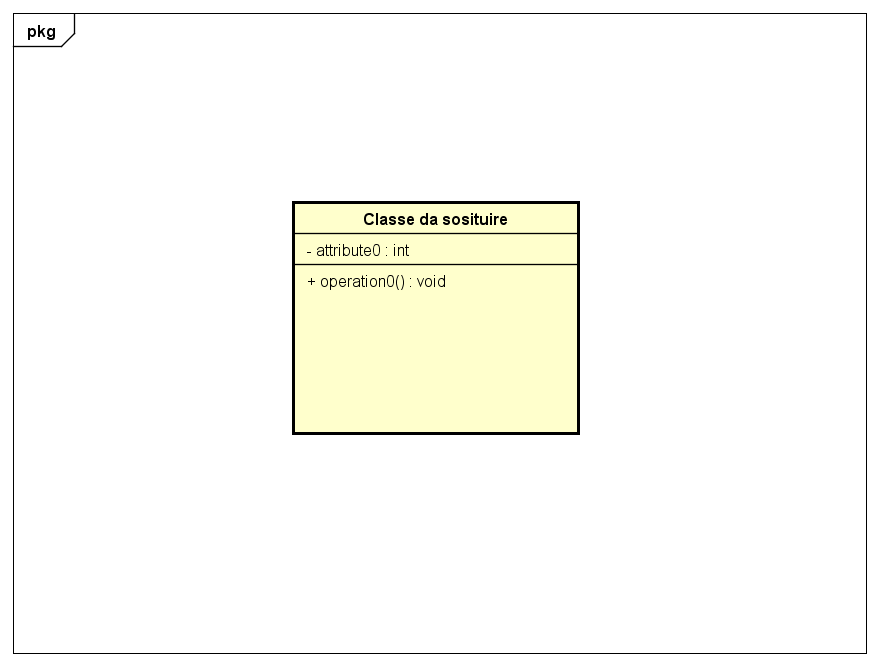
\includegraphics[scale=0.45]{UML/Classi/Front-End/Temporanea.png}
	\caption{QuizziPedia::Front-End::Controllers::QuestionnaireQuestionsManagementController}
\end{figure}
\begin{itemize}
	\item \textbf{Descrizione}: questa classe permette di gestire il recupero delle domande per il questionario;
	\item \textbf{Utilizzo}: fornisce le funzionalità per il recupero delle domande dal back-end e le rende disponibili per poter popolare le view;
	\item \textbf{Relazione con altre classi:}
	\begin{itemize}
		\item \textit{IN} \texttt{QuestionnaireQuestionsManagementDirective}: 
		\item \textit{IN} \texttt{QuestionsService}: 
	\end{itemize}
	\item \textbf{Attributi:}
	\begin{itemize}
		\item 
	\end{itemize}
	\item \textbf{Metodi:}
	\begin{itemize}
		\item 
	\end{itemize}
\end{itemize}

\paragraph{QuizziPedia::Front-End::Controllers::InputToListController}
\begin{figure}
	\centering
	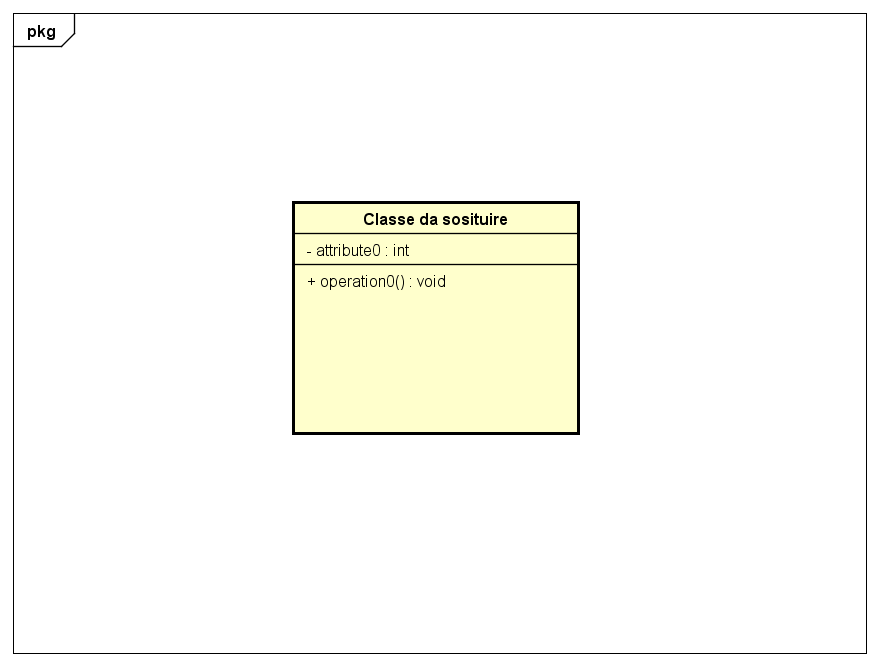
\includegraphics[scale=0.45]{UML/Classi/Front-End/Temporanea.png}
	\caption{QuizziPedia::Front-End::Controllers::InputToListController}
\end{figure}
\begin{itemize}
	\item \textbf{Descrizione}: questa classe permette di gestire la creazione di una domanda, andando ad inserire una porzione di domanda, dopo che è stata confermata, nella parte inferiore della view;
	\item \textbf{Utilizzo}: fornisce le funzionalità per confermare porzioni di domanda durante la creazione;
	\item \textbf{Relazione con altre classi:}
	\begin{itemize}
		\item \textit{IN} \texttt{ConnectionQuestionsView}:
		\item \textit{IN} \texttt{StringsSortingQuestionsView}:  
		\item \textit{IN} \texttt{ImagesSortingQuestionsView}:    
	\end{itemize}
	\item \textbf{Attributi:}
	\begin{itemize}
		\item 
	\end{itemize}
	\item \textbf{Metodi:}
	\begin{itemize}
		\item 
	\end{itemize}
\end{itemize}

\paragraph{QuizziPedia::Front-End::Controllers::NewQuestionsButtonController}
\begin{figure}
	\centering
	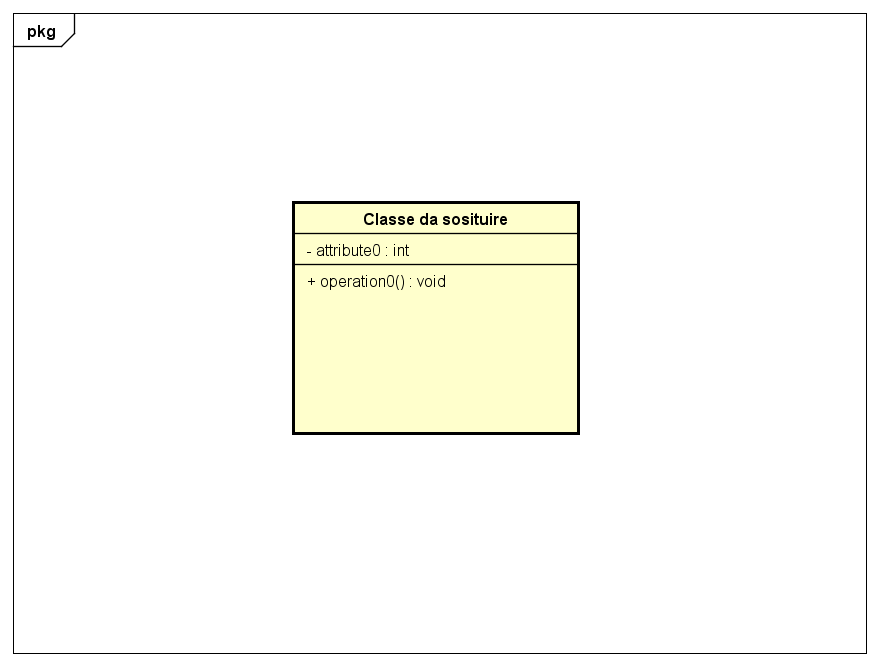
\includegraphics[scale=0.45]{UML/Classi/Front-End/Temporanea.png}
	\caption{QuizziPedia::Front-End::Controllers::NewQuestionButtonController}
\end{figure}
\begin{itemize}
	\item \textbf{Descrizione}: questa classe permette di effettuare il redirect alla pagina di creazione nuova domanda;
	\item \textbf{Utilizzo}: effettua il redirect alla pagina di creazione nuova domanda quando l'utente seleziona l'apposito link;
	\item \textbf{Relazione con altre classi:}
	\begin{itemize}
		\item \textit{IN} \texttt{NewQuestionButtonsDirective} 
	\end{itemize}
	\item \textbf{Attributi:}
	\begin{itemize}
		\item 
	\end{itemize}
	\item \textbf{Metodi:}
	\begin{itemize}
		\item 
	\end{itemize}
\end{itemize}

\paragraph{QuizziPedia::Front-End::Controllers::StatisticsController}
\begin{figure}
	\centering
	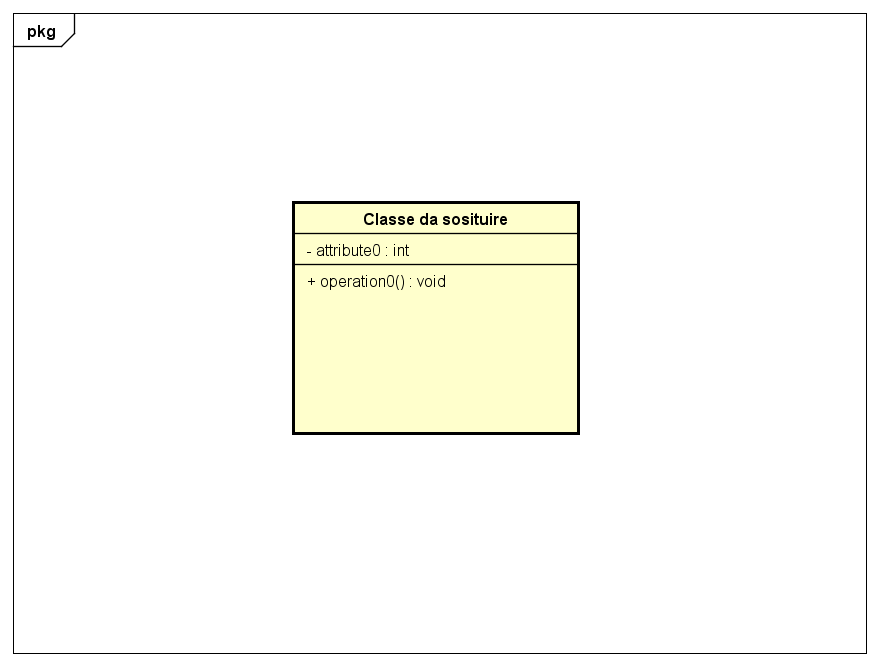
\includegraphics[scale=0.45]{UML/Classi/Front-End/Temporanea.png}
	\caption{QuizziPedia::Front-End::Controllers::StatisticsController}
\end{figure}
\begin{itemize}
	\item \textbf{Descrizione}: questa classe permette di le statistiche di un utente;
	\item \textbf{Utilizzo}: fornisce le funzionalità per ottenere le statistiche di un utente per poterle mostrare nella view;
	\item \textbf{Relazione con altre classi:}
	\begin{itemize}
		\item \textit{IN} \texttt{StatisticsDirective} 
		\item \textit{OUT} \texttt{StatisticsService} 
	\end{itemize}
	\item \textbf{Attributi:}
	\begin{itemize}
		\item 
	\end{itemize}
	\item \textbf{Metodi:}
	\begin{itemize}
		\item 
	\end{itemize}
\end{itemize}

\paragraph{QuizziPedia::Front-End::Controllers::QuizEventController}
\begin{figure}
	\centering
	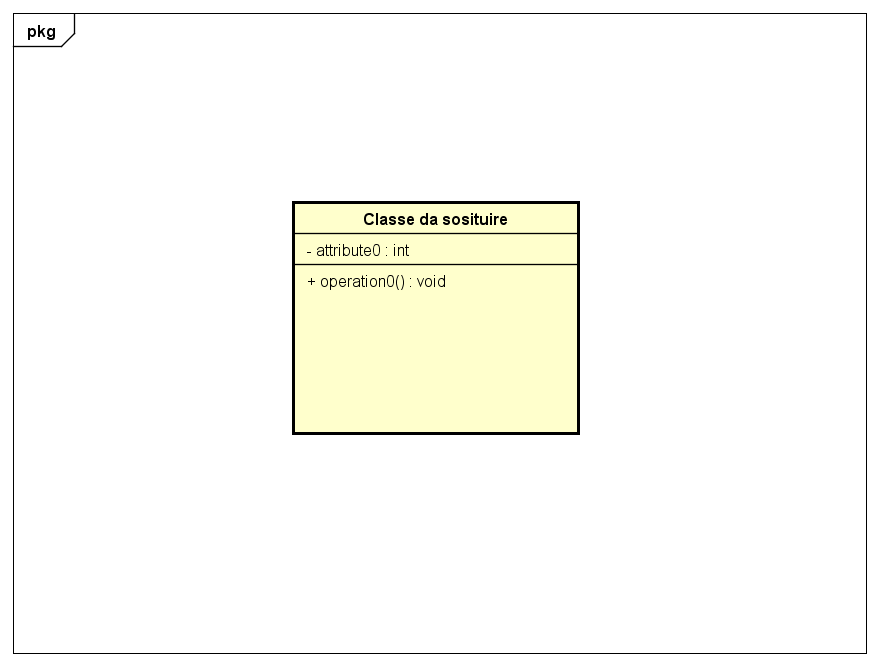
\includegraphics[scale=0.45]{UML/Classi/Front-End/Temporanea.png}
	\caption{QuizziPedia::Front-End::Controllers::QuizEventController}
\end{figure}
\begin{itemize}
	\item \textbf{Descrizione}: questa classe permette di reagire ai comandi dell'utente durante la gestione dei suoi questionari;
	\item \textbf{Utilizzo}: fornisce le funzionalità per reagire ai comandi dell'utente, effettua redirect alle pagine richieste, come la visualizzazione delle statistiche di un questionario e iniziare un questionario in modalità esame.
	\item \textbf{Relazione con altre classi:}
	\begin{itemize}
		\item \textit{IN} \texttt{QuizCreatedDirective} 
		\item \textit{OUT} \texttt{QuizNoExamModeDirective} 
		\item \textit{OUT} \texttt{QuizExamModeDirective} 
	\end{itemize}
	\item \textbf{Attributi:}
	\begin{itemize}
		\item 
	\end{itemize}
	\item \textbf{Metodi:}
	\begin{itemize}
		\item 
	\end{itemize}
\end{itemize}